\section{Project Initialization and Folder Structure}

In this chapter we will guide you through your first steps with {\twodx}. You will create your first project and you will learn how to import micrographs.

\subsection{Launching {\twodx} and Creating a New Project}
Once you installed {\twodx} as described in \autoref{sec:install} you have a {\twodx}-icon in your Applications folder on a Mac or under the Education menu entry under Linux. In case you compiled {\twodx} yourself please launch {\twodx}\texttt{\_merge} in the \texttt{/bin} directory of your installation location. Clicking on this icon will launch {\twodx}\texttt{\_merge} which is the entry point for all {\twodx}-projects. {\twodx} immediately asks you to select your project directory as shown in \autoref{fig:launch_mac}.

\begin{figure}[H]
	\centering
	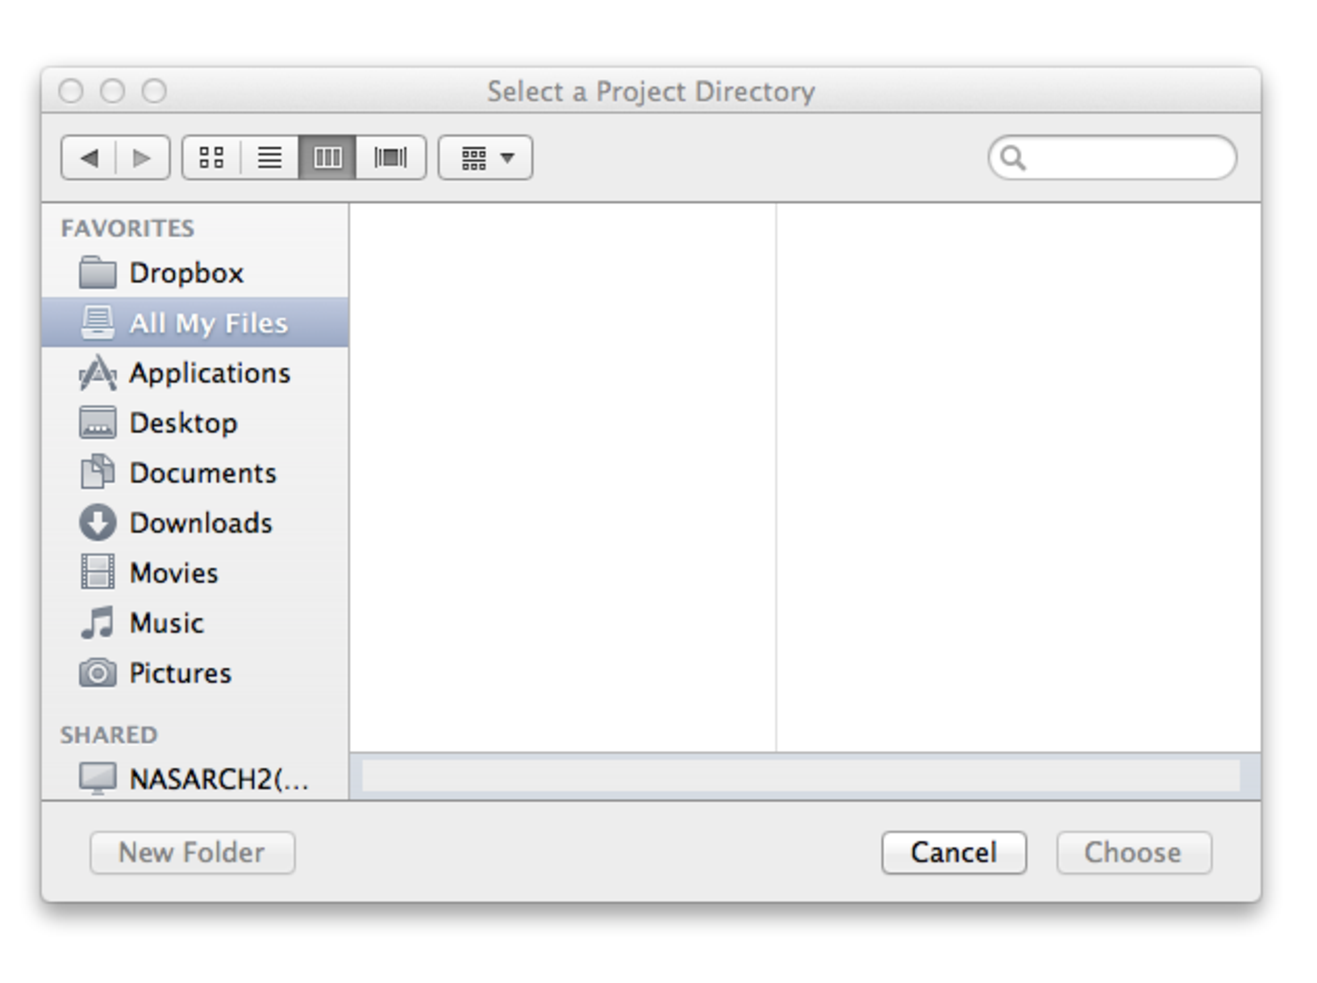
\includegraphics[width=.85\textwidth]{2dx_init_mac.pdf}
	\caption{Launching {\twodx}}
	\label{fig:launch_mac}
\end{figure}

As you don't have a project right now, you should create a new folder called "Protein\_A" under "Desktop". Select the newly generated folder and click on "Choose". {\twodx} now will look for configuration data in the selected folder. If the required data is not found the application will ask you whether a new configuration file should be created in this location as shown in \autoref{fig:create_dir}. For detailed information on the project structure we refer to \autoref{sec:project_struc}.

\begin{figure}[H]
	\centering
	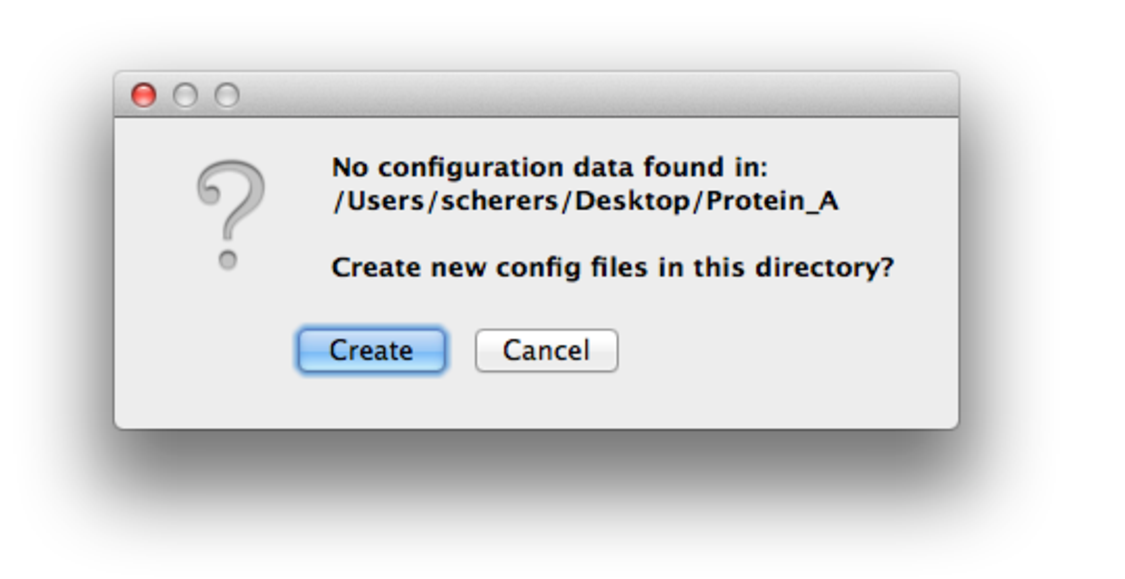
\includegraphics[width=.85\textwidth]{create_dir.pdf}
	\caption{Creating project directory}
	\label{fig:create_dir}
\end{figure}

After the project initialization {\twodx}\texttt{\_merge} will open and you will see the following window shown in \autoref{fig:2dx_merge_gui}. We will discuss all parts of the {\twodx} graphical user interface in \autoref{sec:2dx_merge} and \autoref{sec:2dx_image}.

\begin{figure}[H]
	\centering
	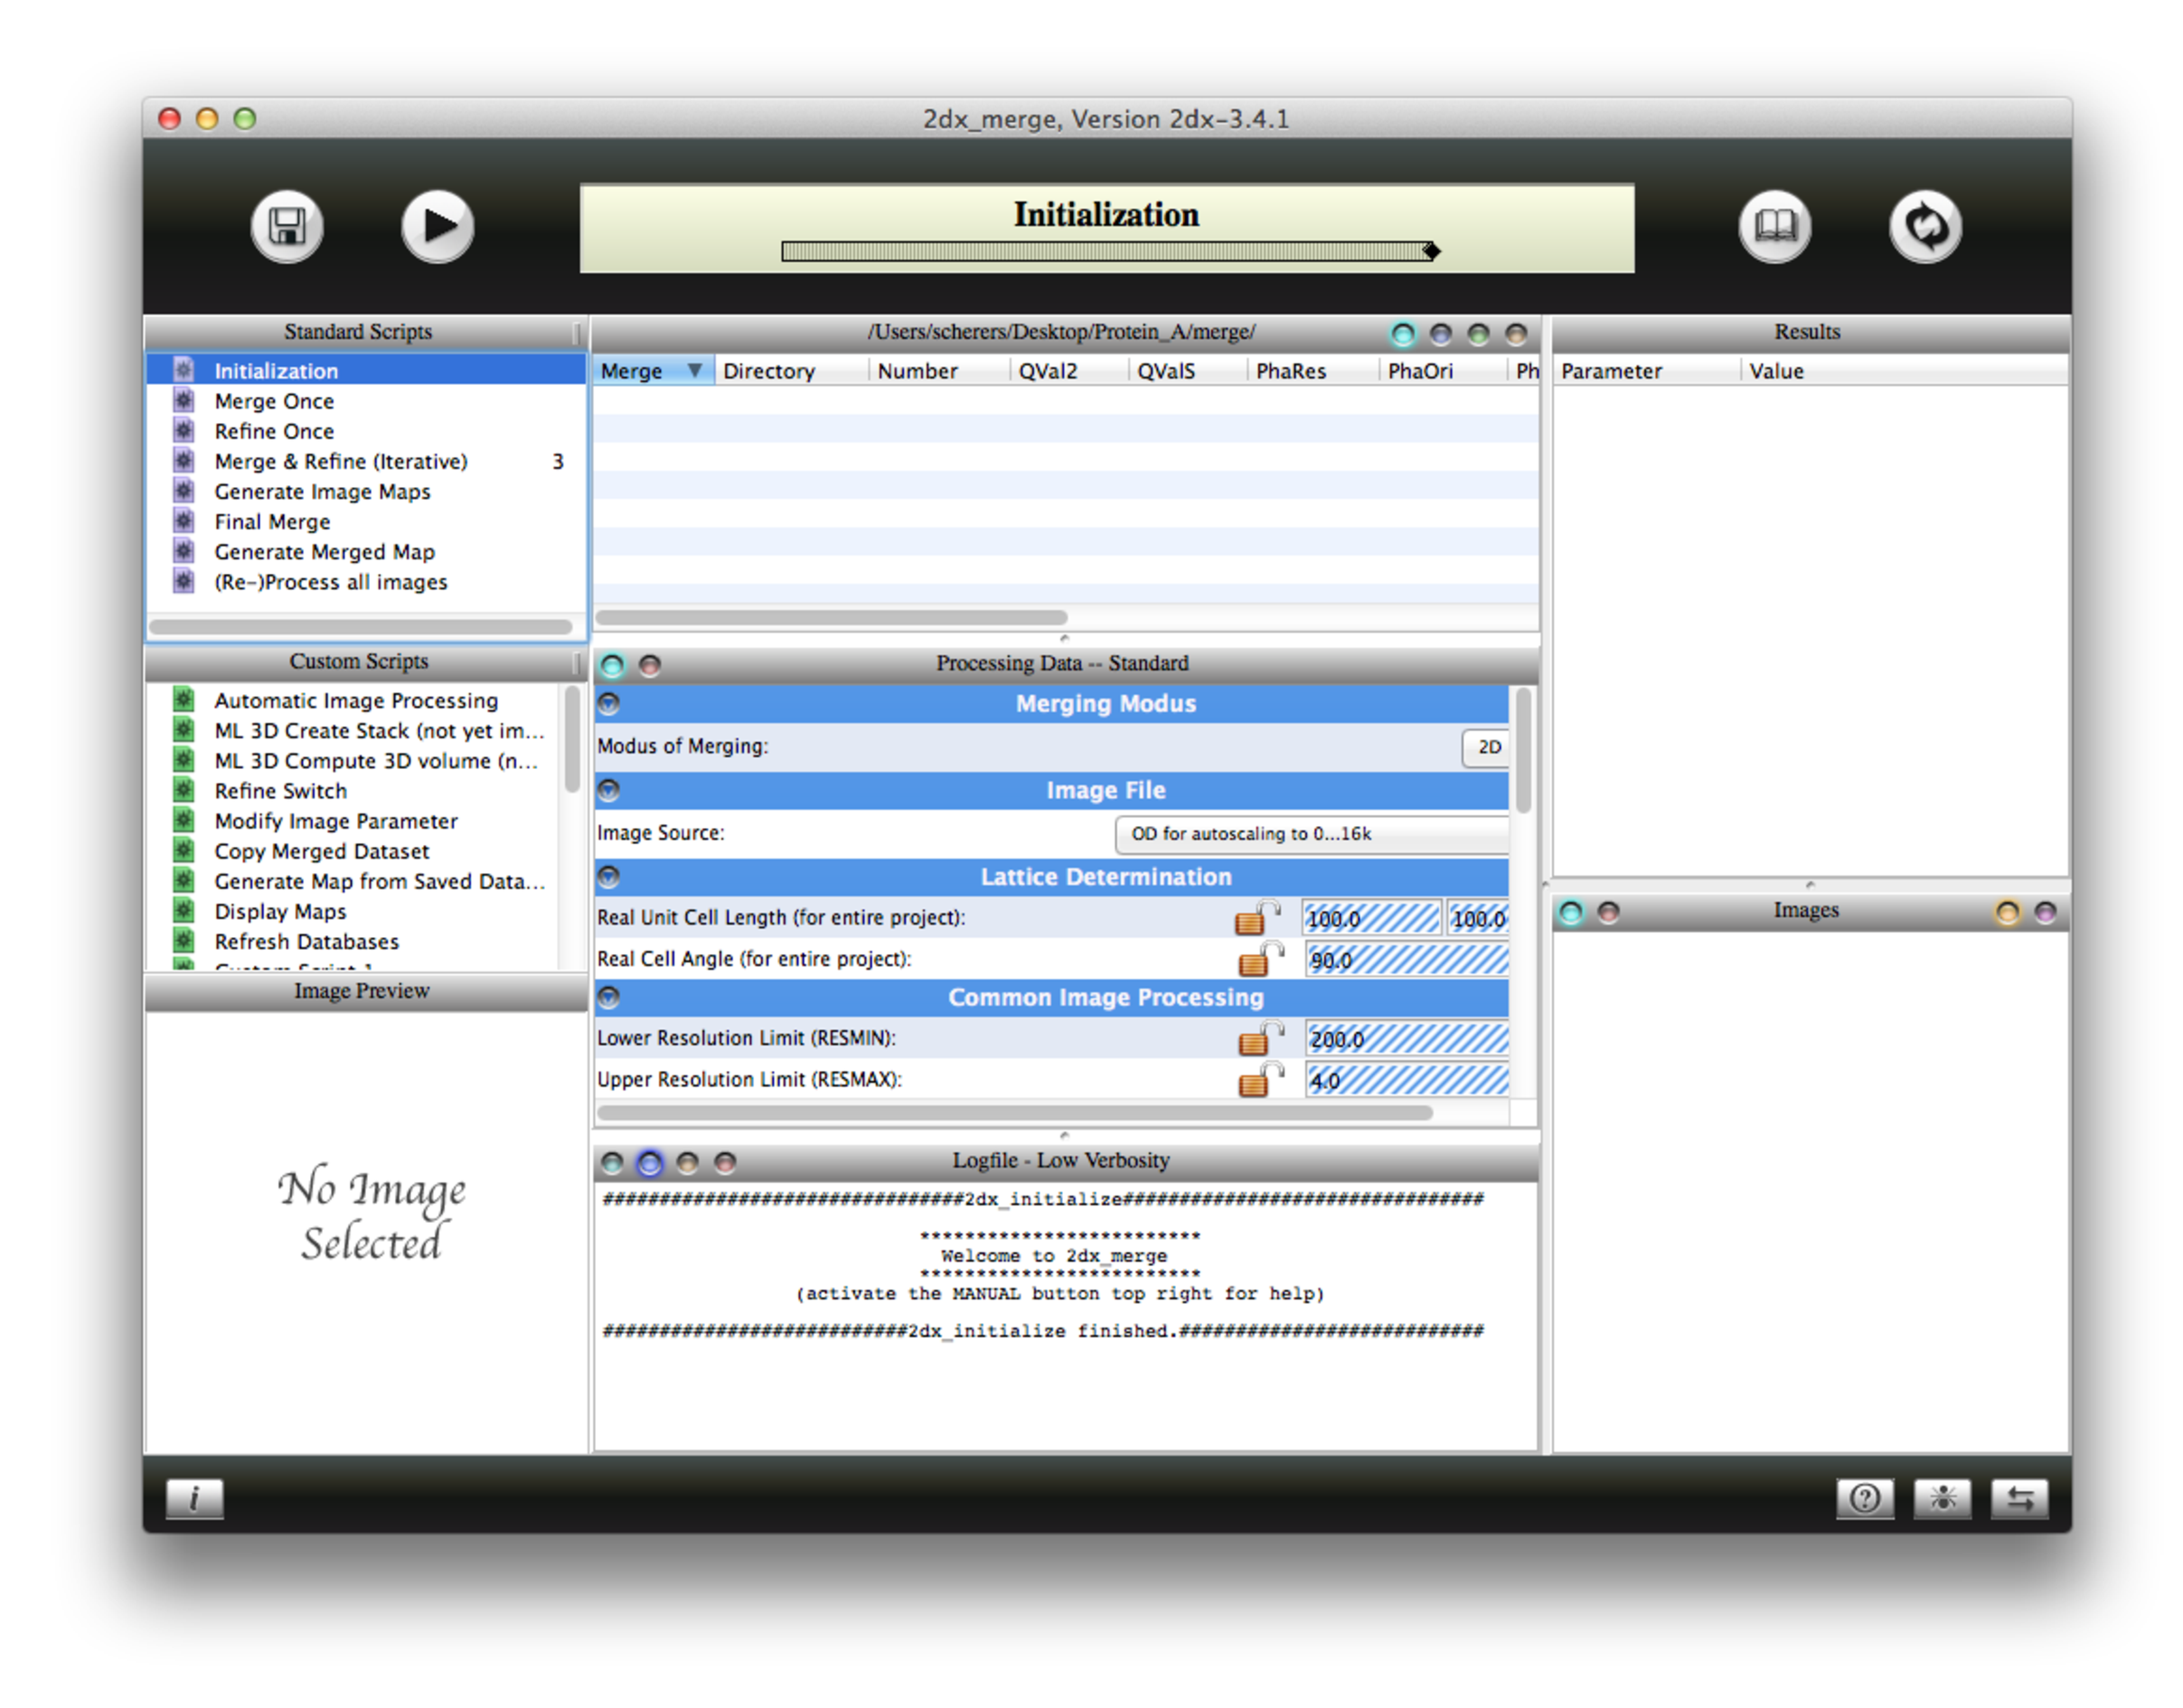
\includegraphics[width=1.0\textwidth]{2dx_merge_gui.pdf}
	\caption{{\twodx} merge GUI}
	\label{fig:2dx_merge_gui}
\end{figure}

So far you have initialized a new {\twodx}-project on your computer and now we are ready to import the first micrographs.

\subsection{Importing Images to {\twodx}}
\label{sec:import}

The whole tutorial you are holding in your hands is based on one exemplary dataset, which you can download from our homepage (\url{http://www.2dx.unibas.ch/download/2dx-software/test-data}). Thus you are encouraged to download the archive to your hard disk. After the download you have to uncompress the archive in order to be able to import the micrographs. 

To import the images into {\twodx} you have to click on "File > Import Images..." in the toolbar at the top of your desktop (\autoref{fig:file_import}).

\begin{figure}[H]
	\centering
	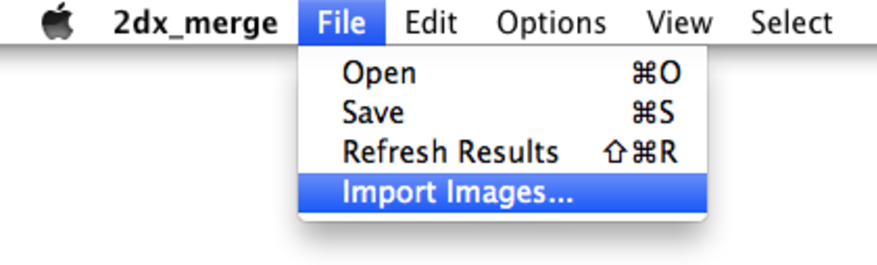
\includegraphics[width=.85\textwidth]{file_import.pdf}
	\caption{Importing files}
	\label{fig:file_import}
\end{figure}

"Import Images..." will open a file browser which is used to navigate to the folder containing the micrographs to import. Once you selected all the micrographs as shown in \autoref{fig:select_files} click on "Open". {\twodx} allows you to import \textit{.tiff} and \textit{.mrc} images. If your data is stored in another format you have to convert your images by means of an external program.
\index{Image format!mrc}
\index{Image format!tiff}

\begin{figure}[H]
	\centering
	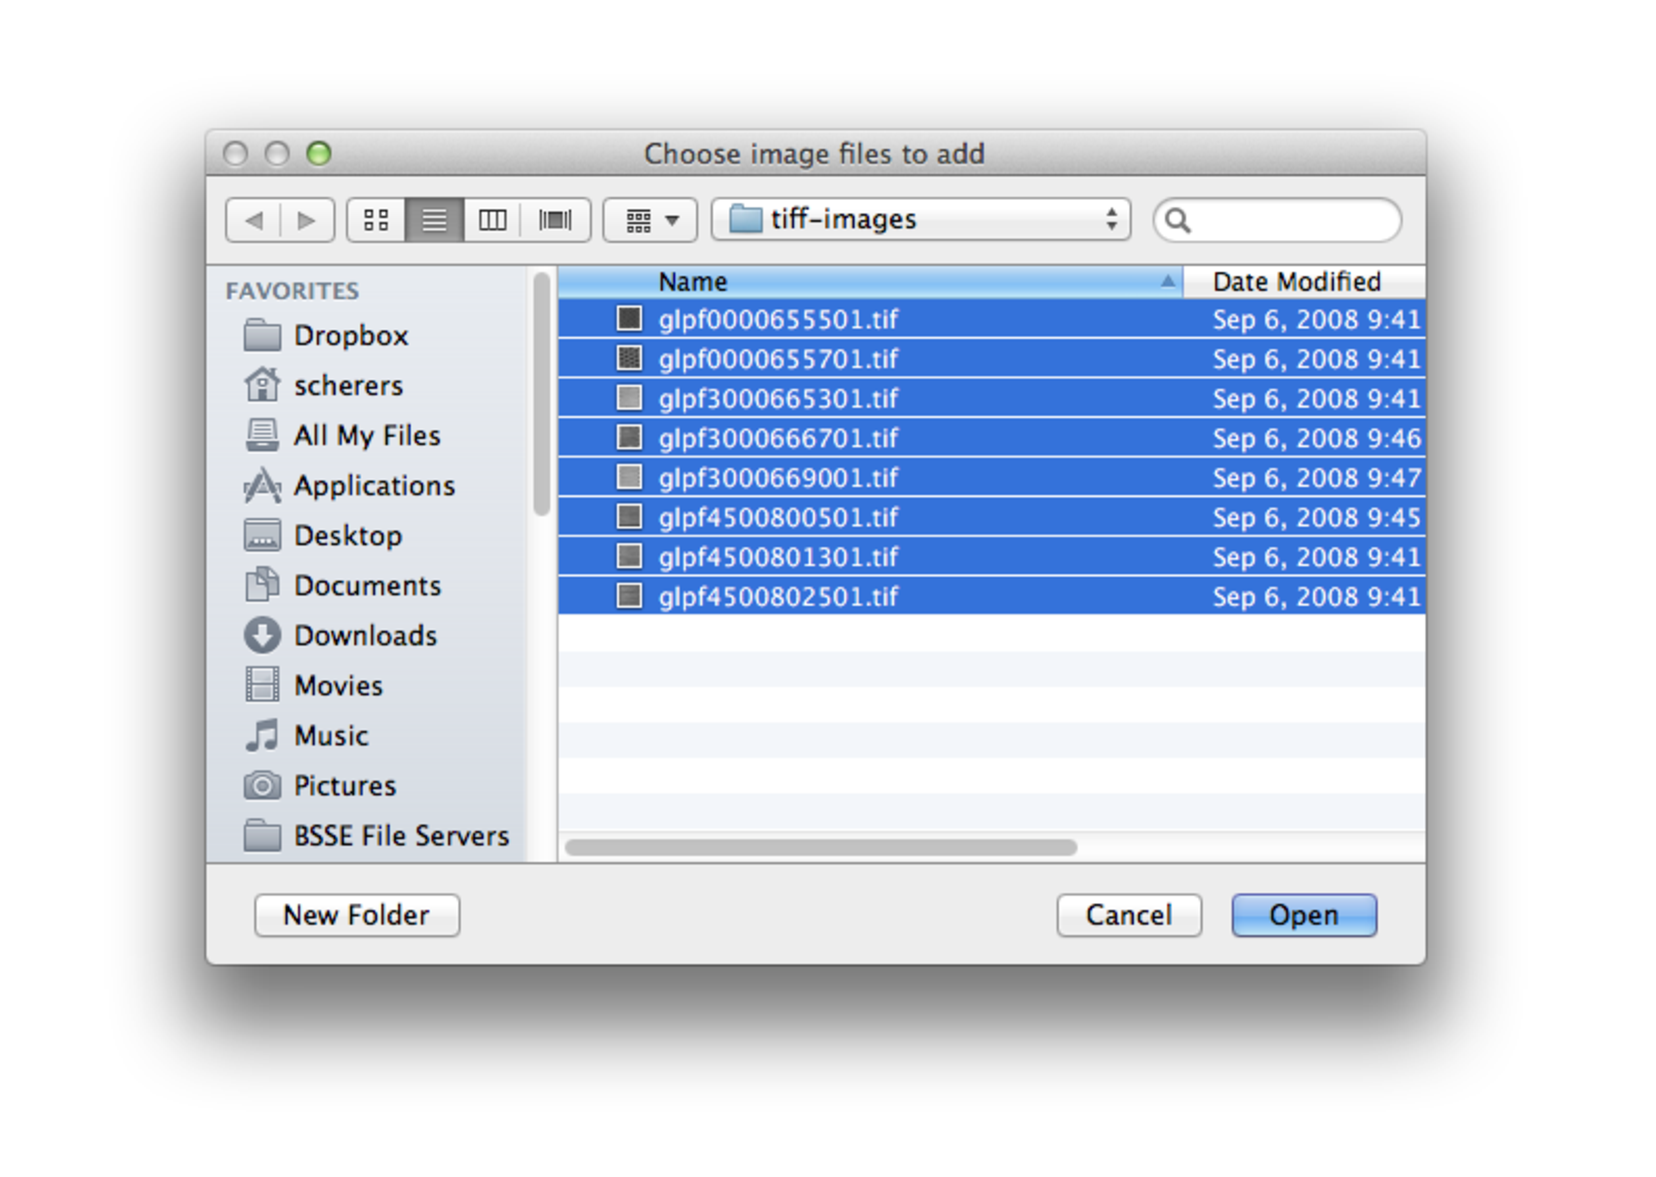
\includegraphics[width=.85\textwidth]{select_files.pdf}
	\caption{Select files to import}
	\label{fig:select_files}
\end{figure}

Usually each electron microscopy lab has a naming convention for their micrographs, which contains additional information about each micrograph, e.g. tilt angle. For instance in our lab the first four letters of an image name are used to store the name of the protein. The following two digits are the tilt angle followed by the six digits image number. The two last digits represent the sub-image number, which usually is set to \texttt{01}. 

The dialog shown in \autoref{fig:import_dialog} allows you to parse the additional image information from the filename. In the left panel of the new dialog all images which will be imported are listed. When finally importing the selected images {\twodx} applies the \textit{regular expression} \index{Regular expression} selected from the pull-down menu in top of the dialog in order to extract the additional information. The right panel of the dialog shown you a preview of the actually parsed information. For the provided test dataset the default regular expression works fine and clicking on "OK" imports the images. You can change the applied expression to your needs and click on "+" in order to store the expression for a later reuse. Details on regular expressions are discussed in \autoref{sec:regexp}.

\begin{figure}[H]
	\centering
	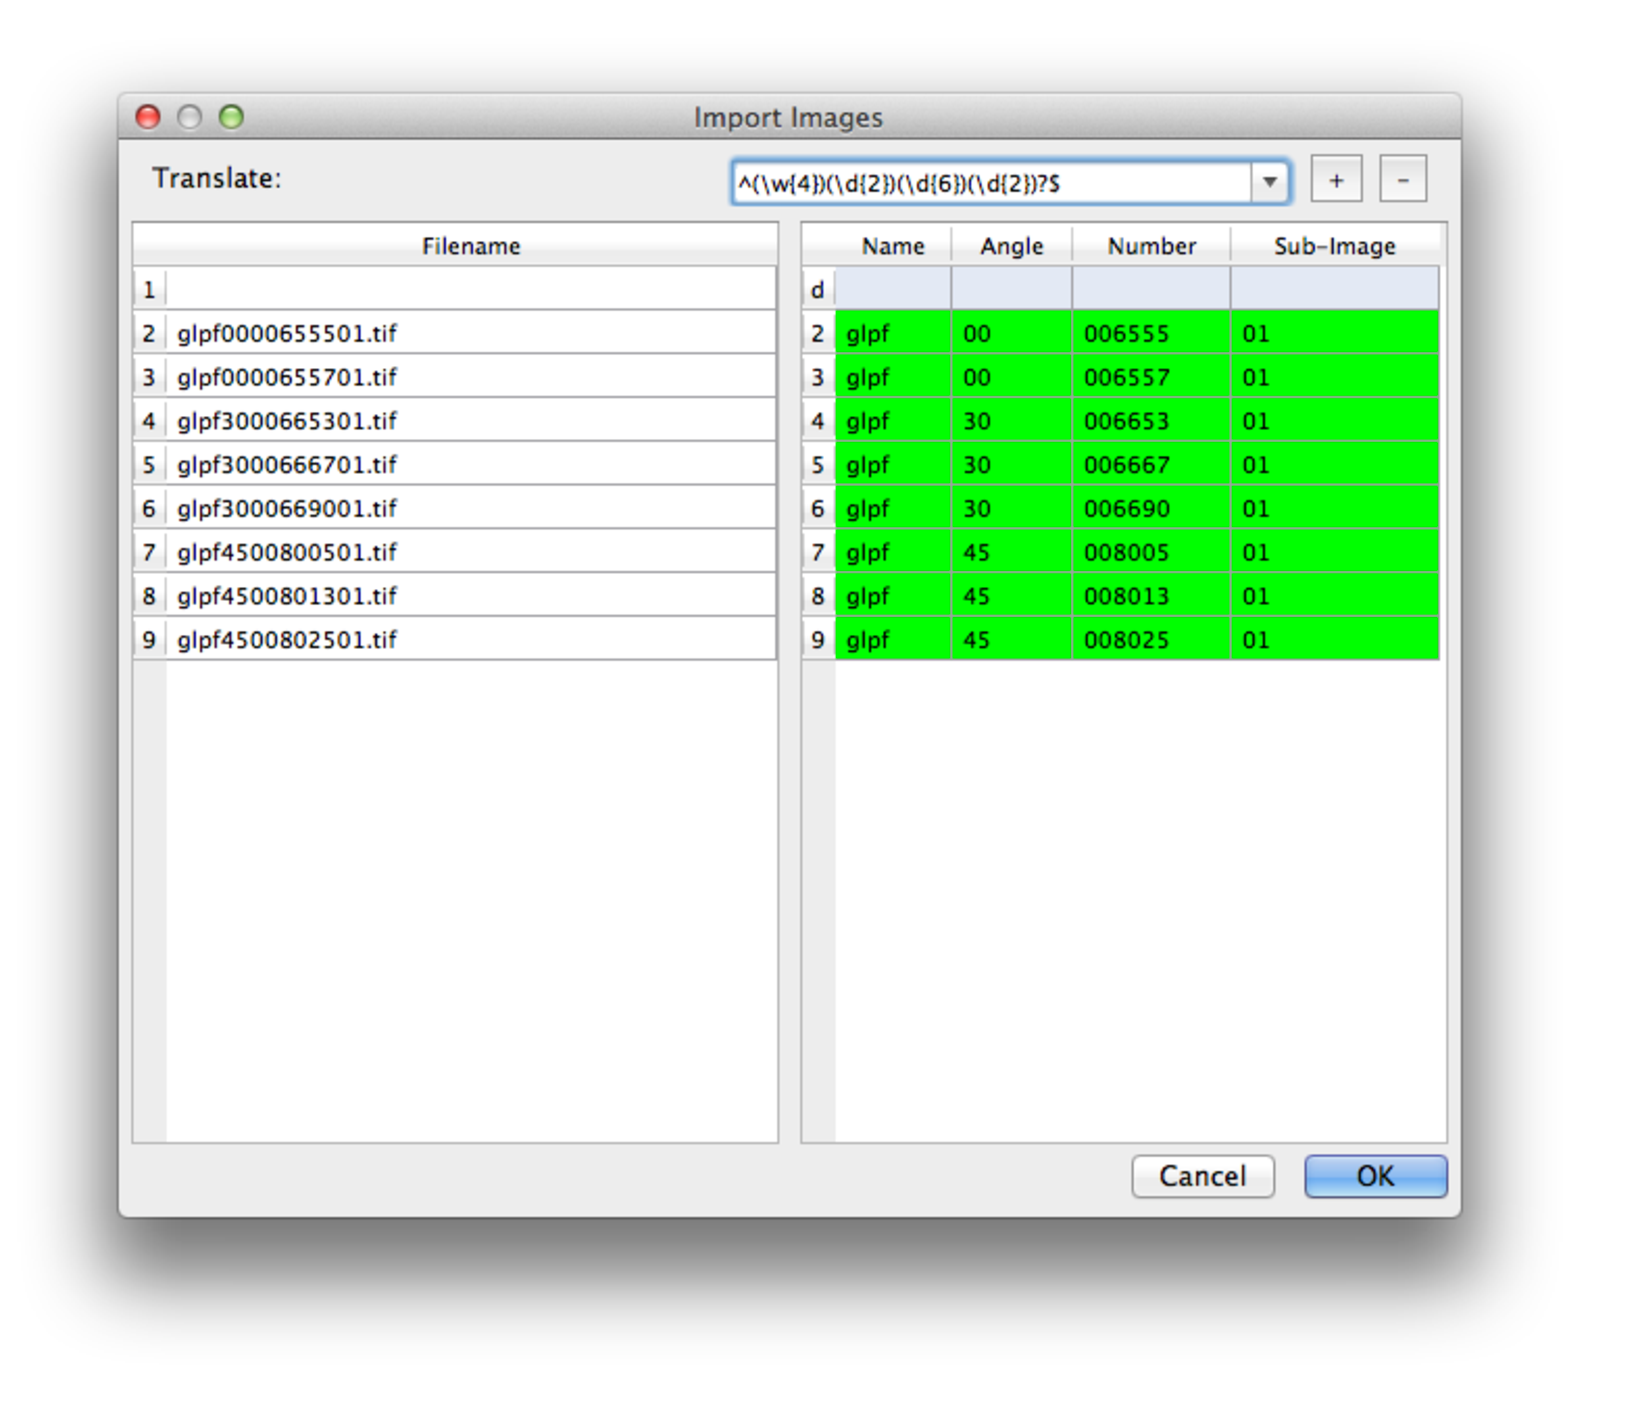
\includegraphics[width=.85\textwidth]{import_dialog.pdf}
	\caption{File import dialog}
	\label{fig:import_dialog}
\end{figure}

Once you imported the images the central panel of the {\twodx} user interface will look like shown in \autoref{fig:imported_images}. 

\begin{figure}[H]
	\centering
	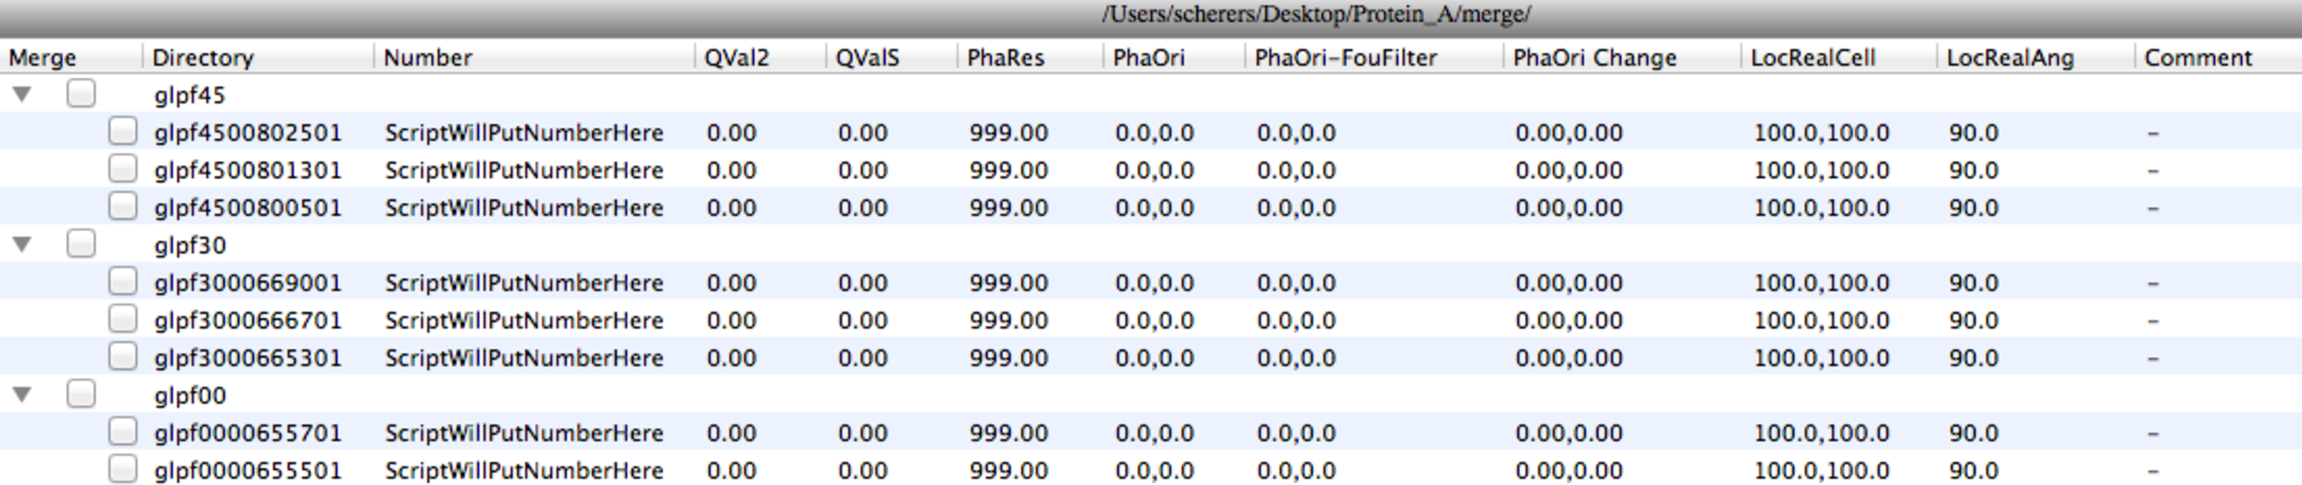
\includegraphics[width=.85\textwidth]{imported_images.pdf}
	\caption{Project panel with imported micrographs}
	\label{fig:imported_images}
\end{figure}

Note that the images are grouped by their name and tilt angle into different tilt series. Before we start processing the individual image we discuss the graphical user interfaces of {\twodx} and some useful technical details in the subsequent \autoref{sec:gui}.

